\documentclass[tikz,border=5pt]{standalone}
\usepackage{fontspec}
\setmainfont{Times New Roman}
\usepackage{unicode-math}
\setmathfont{Cambria Math}
\usetikzlibrary{shapes.geometric,shapes.misc,positioning,fit,backgrounds,arrows.meta,calc}

\begin{document}
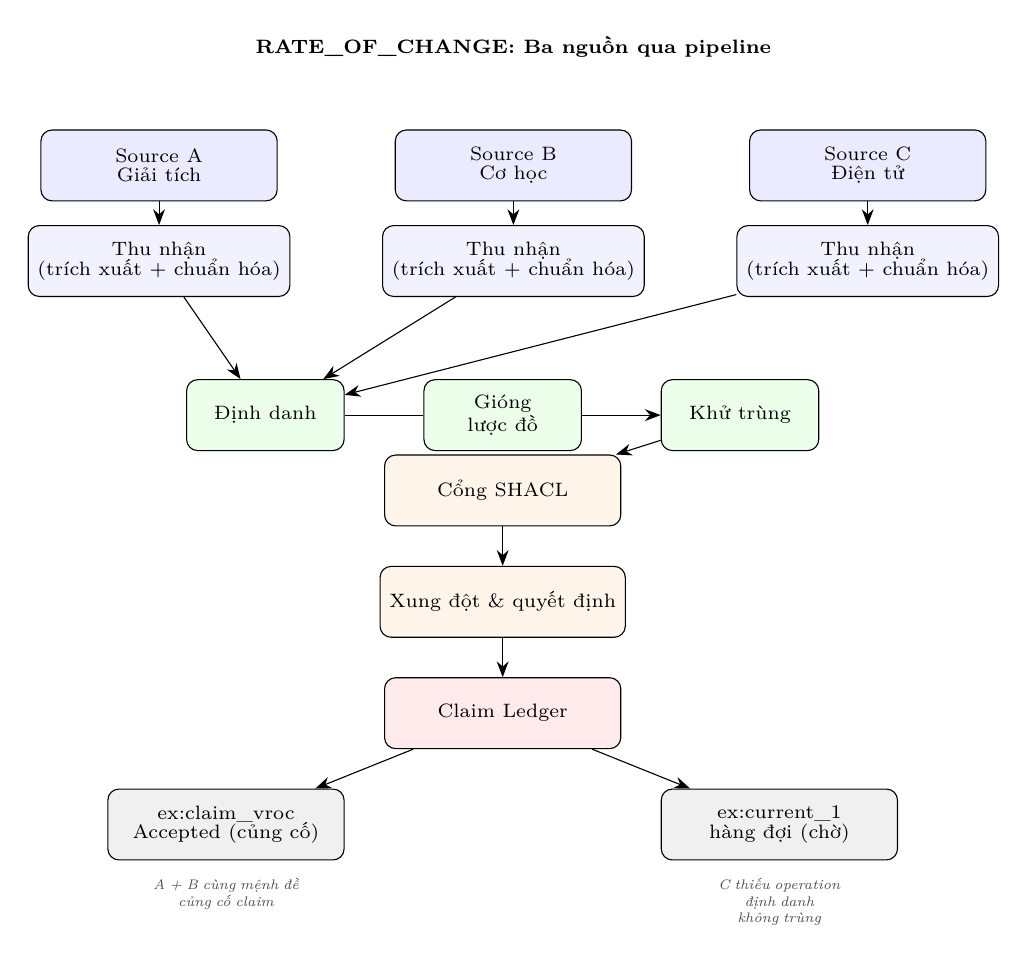
\begin{tikzpicture}[
    node distance=0.8cm and 1.0cm,
    box/.style={rectangle, draw, minimum width=2.2cm, minimum height=0.7cm, align=center, font=\tiny},
    big/.style={rectangle, rounded corners, draw, minimum width=3.0cm, minimum height=0.9cm, align=center, font=\scriptsize},
    arrow/.style={-{Stealth[length=2mm]}, thin},
    label/.style={font=\tiny\itshape, text=gray!60!black},
    phase/.style={font=\scriptsize\bfseries},
]

% Title
\node[phase] at (0, 6.0) {RATE\_OF\_CHANGE: Ba nguồn qua pipeline};

% ====== Sources ======
\node[big, fill=blue!8] (srcA) at (-4.5, 4.5) {Source A\\[-1pt]\scriptsize Giải tích};
\node[big, fill=blue!8] (srcB) at (0, 4.5) {Source B\\[-1pt]\scriptsize Cơ học};
\node[big, fill=blue!8] (srcC) at (4.5, 4.5) {Source C\\[-1pt]\scriptsize Điện tử};

% ====== Acquisition ======
\node[big, fill=blue!5, below=0.3cm of srcA] (acqA) {Thu nhận\\[-1pt]\scriptsize(trích xuất + chuẩn hóa)};
\node[big, fill=blue!5, below=0.3cm of srcB] (acqB) {Thu nhận\\[-1pt]\scriptsize(trích xuất + chuẩn hóa)};
\node[big, fill=blue!5, below=0.3cm of srcC] (acqC) {Thu nhận\\[-1pt]\scriptsize(trích xuất + chuẩn hóa)};

\draw[arrow] (srcA) -- (acqA);
\draw[arrow] (srcB) -- (acqB);
\draw[arrow] (srcC) -- (acqC);

% ====== Integration ======
\node[big, fill=green!8, below=1.5cm of $(acqA)!0.3!(acqB)$, minimum width=2.0cm] (entity) {Định danh};
\node[big, fill=green!8, right=1.0cm of entity, minimum width=2.0cm] (schema) {Gióng\\ lược đồ};
\node[big, fill=green!8, right=1.0cm of schema, minimum width=2.0cm] (dedup) {Khử trùng};

\draw[arrow] (acqA) -- (entity);
\draw[arrow] (acqB) -- (entity);
\draw[arrow] (acqC) -- (entity);
\draw[arrow] (entity) -- (schema) -- (dedup);

% ====== SHACL gate ======
\node[big, fill=orange!8, below=0.5cm of $(entity)!0.5!(dedup)$] (shacl) {Cổng SHACL};
\draw[arrow] (dedup) -- (shacl);

% ====== Decision ======
\node[big, fill=orange!8, below=0.5cm of shacl] (conflict) {Xung đột \& quyết định};
\draw[arrow] (shacl) -- (conflict);

% ====== Ledger ======
\node[big, fill=red!8, below=0.5cm of conflict] (ledger) {Claim Ledger};
\draw[arrow] (conflict) -- (ledger);

% ====== Outcomes ======
\node[big, fill=gray!12, below left=0.5cm and 0.5cm of ledger] (vroc) {ex:claim\_vroc\\[-1pt]\scriptsize Accepted (củng cố)};
\node[big, fill=gray!12, below right=0.5cm and 0.5cm of ledger] (curr) {ex:current\_1\\[-1pt]\scriptsize hàng đợi (chờ)};
\draw[arrow] (ledger) -- (vroc);
\draw[arrow] (ledger) -- (curr);

% ====== Labels ======
\node[label, align=center, text width=2.0cm, below=0.1cm of vroc] {A + B cùng mệnh đề\\củng cố claim};
\node[label, align=center, text width=2.0cm, below=0.1cm of curr] {C thiếu operation\\định danh không trùng};

\end{tikzpicture}
\end{document}